\documentclass{beamer}

\usepackage{hyperref}
\usepackage{graphicx}
\usepackage{caption}
\usepackage{algorithmicx}
\usepackage{algorithm}
\usepackage{algpseudocode}
\usepackage{tikz}
\usetikzlibrary{positioning}

\usetheme{CambridgeUS}
\date{}

\setbeamercolor{block title}{fg=CambridgeRed}

\hypersetup{colorlinks = true, urlcolor = CambridgeRed}


\title[]{Hierarchical Graph Drawing Algorithms}
\author[]{Anish Teja Bramhajosyula}
\institute[]{International Institute of Information Technology Bangalore}

\AtBeginSection[]
{
  \begin{frame}{Outline}
    \tableofcontents[currentsection]
  \end{frame}
}


\definecolor{CambridgeRed}{RGB}{203, 0, 0}
\setbeamercolor{itemize item}{fg=CambridgeRed}
\setbeamercolor{itemize subitem}{fg=CambridgeRed}
\setbeamercolor{itemize subsubitem}{fg=CambridgeRed}
\setbeamercolor{item projected}{bg=CambridgeRed, fg=white}



\begin{document}


% TITLEPAGE
\begin{frame} \titlepage \end{frame}



% INTRODUCTION
\begin{frame}{Introduction}
    
    \begin{itemize}
        
        \item \textbf{\texttt{smcat}} is a complete pipeline to read (supported) statechart modelling languages and render them in specified output formats.

        \item Input formats supported: \texttt{smcat}, \texttt{scxml}, \texttt{json}.
        \item Output formats supported: \texttt{ast}, \texttt{dot}, \texttt{eps}, \texttt{json}, \texttt{oldeps}, \texttt{oldps}, \texttt{oldps2}, \texttt{oldsvg}, \texttt{pdf}, \texttt{png}, \texttt{ps}, \texttt{ps2}, \texttt{scjson}, \texttt{scxml}, \texttt{smcat}, \texttt{svg}.

    \end{itemize}

\end{frame}


% SMCAT PIPELINE
\begin{frame}{Execution Pipeline}
    

    \begin{center}

        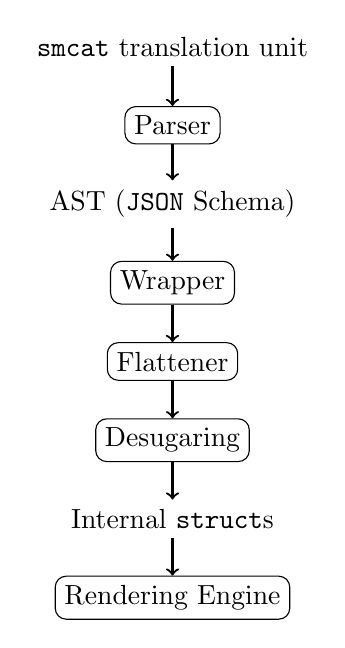
\begin{tikzpicture}
            
            \node[] (input) {\texttt{smcat} translation unit};
            \node[draw, rounded corners, below of=input] (start) {Parser};
            \node[below of=start] (out1) {AST (\texttt{JSON} Schema)};
            \node[draw, rounded corners, below of=out1] (step1) {Wrapper};
            \node[draw, rounded corners, below of=step1] (step2) {Flattener};
            \node[draw, rounded corners, below of=step2] (step3) {Desugaring};
            \node[below of=step3] (out2) {Internal \texttt{struct}s};
            \node[draw, rounded corners, below of=out2] (step4) {Rendering Engine};

            \draw[->, thick] (input) -- (start);
            \draw[->, thick] (start) -- (out1);
            \draw[->, thick] (out1) -- (step1);
            \draw[->, thick] (step1) -- (step2);
            \draw[->, thick] (step2) -- (step3);
            \draw[->, thick] (step3) -- (out2);
            \draw[->, thick] (out2) -- (step4);

        \end{tikzpicture}
    
    \end{center}

\end{frame}



% GRAPHVIZ
\begin{frame}{Graphviz}
    

    \begin{itemize}
        
        \item Graph Visualisation Software developed by AT\&T
        \item Uses a modelling language called \texttt{dot}
        \item Employs various algorithms for layouting the vertices of a graph, assigning physical coördinates and drawing edges suitably

    \end{itemize}


\end{frame}


% GRAPHVIZ PIPELINE
\begin{frame}{Execution Pipeline}
    

    \begin{center}
        
        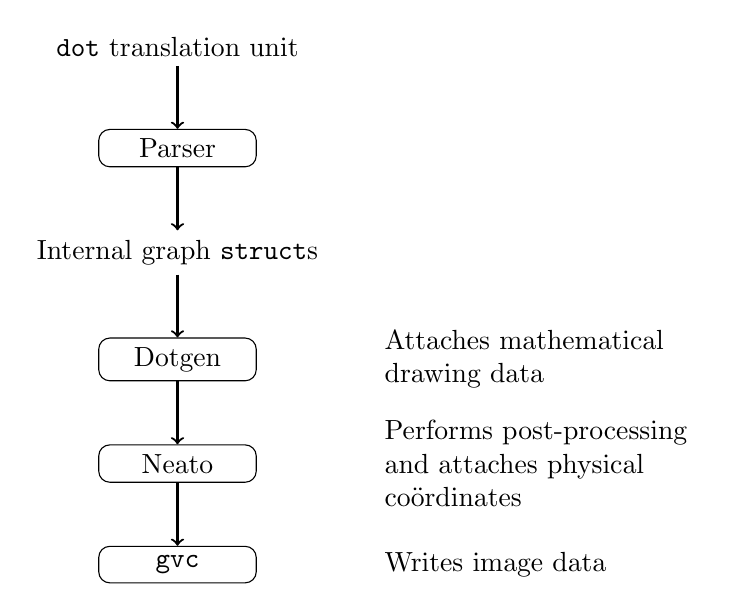
\begin{tikzpicture}[
            node distance=0.8cm and 1.5cm,
            block/.style={draw, rounded corners, minimum width=2cm}
        ]

            \node (input) {\texttt{dot} translation unit};
            \node[block, below=of input] (start) {Parser};
            \node[below=of start] (out1) {Internal graph \texttt{struct}s};
            \node[block, below=of out1] (step1) {Dotgen};
            \node[block, below=of step1] (step2) {Neato};
            \node[block, below=of step2] (step3) {\texttt{gvc}};


            \node[right=of step1, text width=4cm] (note1) {Attaches mathematical drawing data};
            \node[right=of step2, text width=4cm] (note2) {Performs post-processing and attaches physical coördinates};
            \node[right=of step3, text width=4cm] (note3) {Writes image data};

            \draw[->, thick] (input) -- (start);
            \draw[->, thick] (start) -- (out1);
            \draw[->, thick] (out1)  -- (step1);
            \draw[->, thick] (step1) -- (step2);
            \draw[->, thick] (step2) -- (step3);

        \end{tikzpicture}

    \end{center}

\end{frame}



% DOTGEN
\begin{frame}{Dotgen}


    \begin{itemize}

        \item Converts to directed acyclic graph (DAG)
        \item Utilises the Sugiyama framework:


        \begin{itemize}
        
            \item Vertex Ranking/Levelling (assign vertices to levels)
            \item Minimise number of edge crossings
            \item Straighten the edges — route the edges and calculate coördinates

        \end{itemize}

        \item Passes resulting data to \texttt{neato} to attach physical coördinates

    \end{itemize}
    

\end{frame}


% SUGIYAMA FRAMEWORK
\begin{frame}{Sugiyama Framework}
    

    \textbf{Goal}: Given a directed acyclic graph (DAG):

    \begin{enumerate}
        
        \item Edges must point in a uniform direction.
        \item Short \& straight edges are more readable.
        \item Uniformly distributed vertices avoid clutter.
        \item Edge crossings obstruct comprehension.

    \end{enumerate}


\end{frame}


% SUGIYAMA EXAMPLE
\begin{frame}{Example graph drawn using the Sugiyama framework}
    
    \begin{center}
        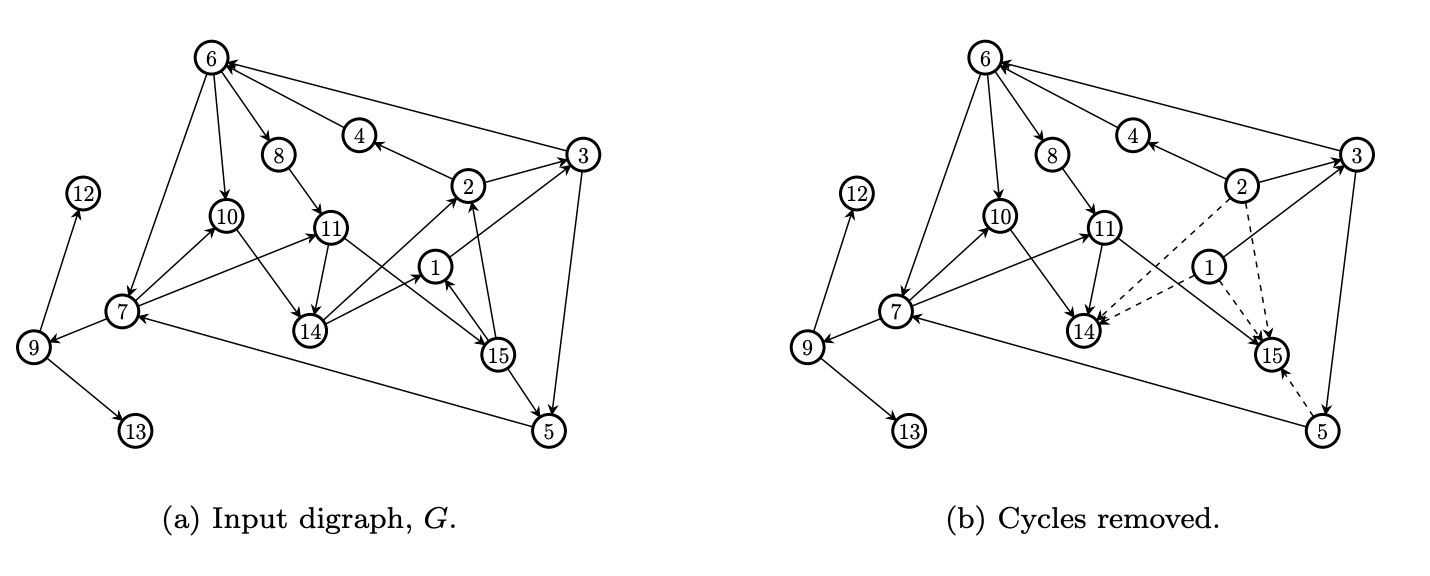
\includegraphics[scale = 0.45]{sugiyama1.png}
    \end{center}

\end{frame}

\begin{frame}{Example graph drawn using the Sugiyama framework}
    
    \begin{center}
        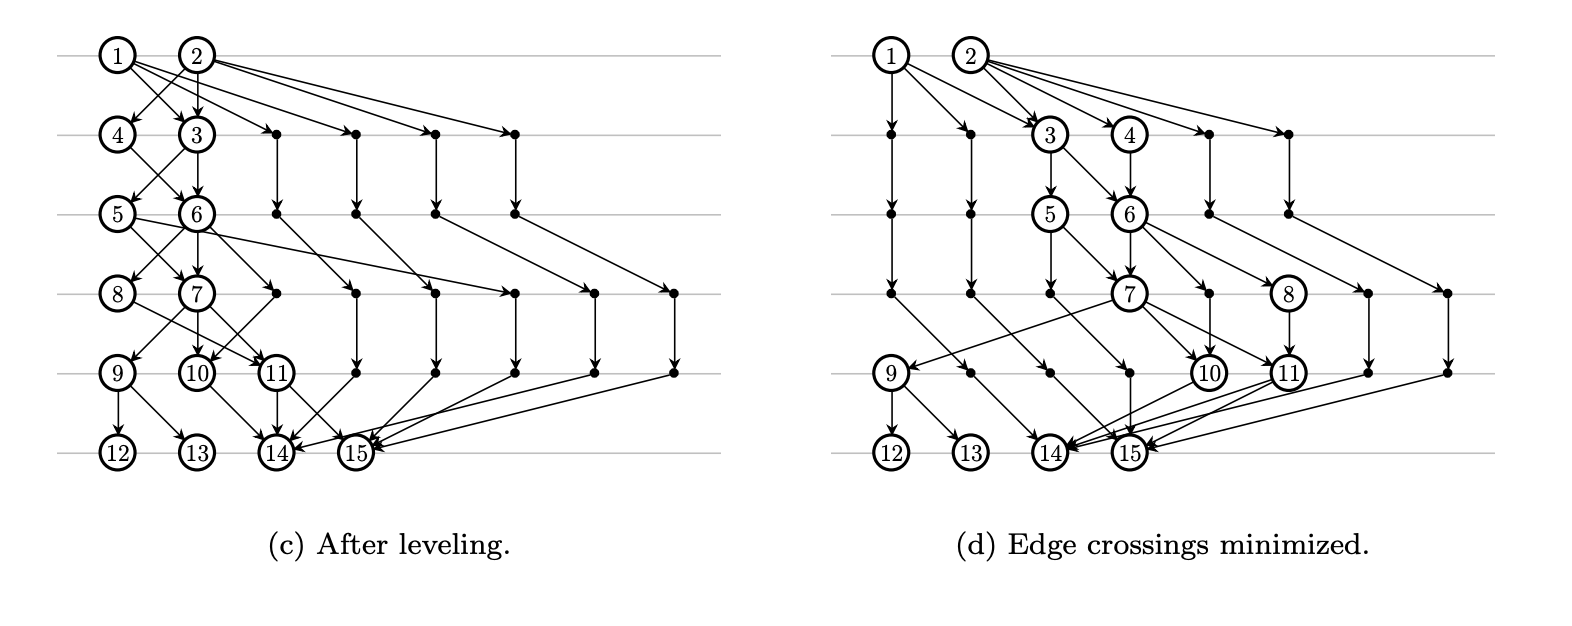
\includegraphics[scale = 0.45]{sugiyama2.png}
    \end{center}

\end{frame}

\begin{frame}{Example graph drawn using the Sugiyama framework}
    
    \begin{center}
        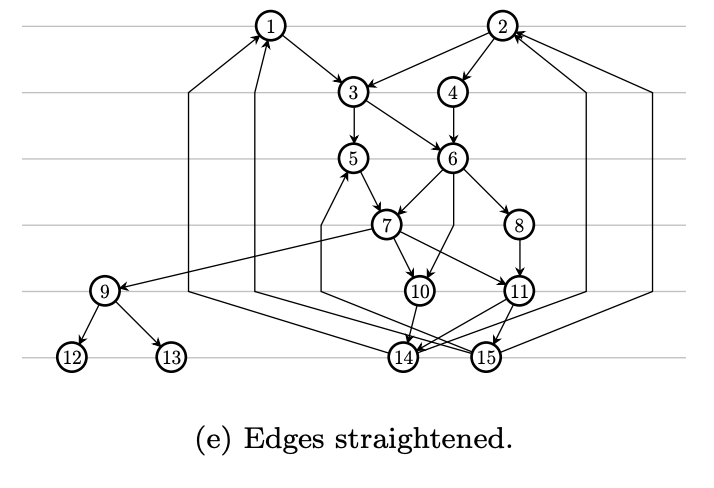
\includegraphics[scale = 0.75]{sugiyama3.png}
    \end{center}

\end{frame}

% SUGIYAMA PREPROCESSING
\begin{frame}{Cycle Removal — Preprocessing}


    \begin{definition}
        
        A graph $(V, E)$ has a \textbf{\textit{two–cycle}} if $\exists u,v \in V : (u,v) \in E \land (v,u) \in E$

    \end{definition}

    
    \begin{itemize}
        
        \item It is assumed that the input digraph has no two–cycles.
        \item While the \texttt{dotgen} engine removes offending edges which make the digraph cyclic, it is an extension to the theoretical framework, and is feasible because the removed edges only affect its internal rendering and not the actual graph itself and can be added back later. In the theoretical model, offending edges are only reversed, since working on a subgraph of the original digraph (with missing edges) may have undesirable results.


    \end{itemize}

\end{frame}


\begin{frame}

    \begin{definition}
        
        A set of edges whose removal makes a digraph acylic is called a \textbf{\textit{Feedback Arc Set} (FAS).}

    \end{definition}

    \begin{definition}
        
        A set of edges whose reversal makes a digraph acyclic is called a \textbf{\textit{Feedback Set} (FS).}

    \end{definition}


\end{frame}


\begin{frame}
    

    \begin{lemma}

        Given an edge set $E$, if $E_0 \subseteq E$ is an FS, then $E_0$ is also an FAS.

    \end{lemma}

    \begin{proof}

        We prove by contradiction. Let $G := (V, E)$ be the original graph, $G_{FS}$ be the graph obtained by reversing the edges in $E_0$, and $G_{FAS}$ be the graph obtained by removing the edges in $E_0$.

        Suppose that $E_0$ is an FS, i.e, $G_{FS}$ is a DAG, but $E_0$ is not an FAS, hence $G_{FAS}$ is not a DAG, i.e., it contains at least one directed cycle, say $C$.

        Let $E_1$ be the set of edges in $E_0$ with reversed directions. Then, the edge set of $G_{FS}$ is $(E \setminus E_0) \cup E_1$.

        $\because E \setminus E_0 \subseteq (E \setminus E_0) \cup E_1 \Rightarrow$ Since $C$ is contained in $G_{FAS}$, all edges of $C$ are in $E \setminus E_0$, hence $C$ must be present in $G_{FS}$ as well.

        But, $G_{FS}$ is a DAG, which is a contradiction.

    \end{proof}

\end{frame}


\begin{frame}
    

    \begin{lemma}
        
        It is always possible and easy to find an FS for a digraph.

    \end{lemma}

    \begin{proof}
        
        This proof can be generalised by induction.

        Suppose $G := (V, E)$ and $V := \{v_1 \dots v_n\}$. Let $(i_1 \dots i_n)$ be any permutation of $(1 \dots n)$ such that we get an arbitrary ordering ($v_{i_1} \dots v_{i_n})$ of $V$. Now, any edge in $E$ must either go forward or backward in this ordering, and cycles are not possible, as opposite directions are partitioned into two different subsets. This partitions $E$ into two sets, say $E_0$ and $E_1$, respectively. If all the edges in one of the subsets is reversed, then all the edges in $E$ point forward, and hence no cycle exists anymore in $G$. Thus, we have converted $G$ to a DAG using a subset of edges (FS) in polynomial time.

    \end{proof}


\end{frame}



\begin{frame}
        

    \begin{itemize}

        \item A typical requirement for an FS is to have the minimum number of edges.
        \item Finding a minimum–cardinality FS, which is equivalent to finding a minimum-cardinality FS, is known to be NP–hard.
        \item We use heuristics to solve these problems.
        \item The following algorithms are based on vertex–ordering:
            
            \begin{itemize}
                
                \item DFS Approach
                \item Vertex Out–Degree Approach
                \item Divide \& Conquer Approach
                \item Berger–Shor Algorithm
                \item Greedy Cycle Removal

            \end{itemize}

        \item A greedy algorithm with heuristics based on breaking cycles edge–by–edge is also covered.

    \end{itemize}
        

\end{frame}


% VERTEX ORDERING HEURISTICS

\begin{frame}{Heuristics based on Vertex–Ordering}
    

    \textbf{Depth–First Search Approach}

    \begin{theorem}[stated without proof]
        
        A digraph has a cycle if and only if its DFS tree has a back edge.

    \end{theorem}

    \begin{itemize}
        
        \item It can be shown that there exist vertex orderings of a digraph for which the FS partitions have the same size.
        \item Hence, such an ordering can be found by performing DFS in linear time.
        \item Based on the above theorem, the back edges in the DFS tree form the FS.
        \item The number of back edges is at most $|E| - |V| + 1$, which is expensive for dense graphs, since $|E| \rightarrow |V|^2$.

    \end{itemize}


\end{frame}



\begin{frame}{Heuristics based on Vertex–Ordering}


    \textbf{Vertex Out–Degree Approach}

    \begin{itemize}

        \item According to Eades \textit{et al.}, 1993, the vertices are ordered from top to bottom, with non–increasing out–degree at every vertex. This ordering can be computed in linear time and is shown to give smaller FSs than the DFS method.

        \item The vertices are partitioned such that all the edges point in one direction in an ordering (in the DAG, using the output FS), so that they naturally \textit{flow} from top to bottom. Hence, we place high out–degree vertices at the top and low at the bottom.

    \end{itemize}


\end{frame}



\begin{frame}[fragile, shrink=7.5]
    \vspace{0.3em}
    \textbf{\Large Divide \& Conquer Approach}
    \vspace{0.5em}

    {\fontsize{3pt}{4pt}\selectfont
    \begin{algorithm}[H]

        \caption*{\textit{Eades\_DAG}} 
        
        \begin{algorithmic}[1]
            \State \textbf{Input:} Graph $G := (V, E)$
            \State \textbf{Output:} FS $V_1, V_2$
            \Statex
            \State Label vertices of $G$ as $\{i, i + 1, \dots, i + |V| - 1\}$

            \Statex
            \Procedure{\textproc{Ordering}}{$V, E, i$} :=

                \If{$|V| = 1$}
                    \State \textproc{label}($V, i$)
                    \State \Return
                \EndIf
                \Statex

                \State $k \gets$ \textbf{if} $|V|$ is even \textbf{then} $\frac{|V|}{2}$ \textbf{else} 1

                \State $V_1, V_2 \gets $ \textproc{partition}($V$) : $\forall v_1 \in V_1, v_2 \in V_2, \Delta^+_G(v_1) \geq \Delta^+_G(v_2)$

                \Statex

                \State \textbf{call} \textproc{ordering}($V_1, E, i$)
                \State \textbf{call} \textproc{ordering}($V_2, E, i + |V_1|$)

            \EndProcedure
        \end{algorithmic}
    \end{algorithm}
    }
\end{frame}


\begin{frame}{Heuristics based on Vertex–Ordering}
    
    \textbf{Divide \& Conquer Approach}

    \begin{itemize}
        
        \item Running Time: $O(\min\{(|V| + |E|)\lg|V|, |V|^2\})$
        \item Observed to produce 20\% better results, especially for dense digraphs

    \end{itemize}

\end{frame}


\begin{frame}[fragile, shrink=7.5]{Heuristics based on Vertex–Ordering}


    {\fontsize{3pt}{4pt}\selectfont
    \begin{algorithm}[H]

        \caption*{\textit{Berger–Shor Algorithm}} 
        
        \begin{algorithmic}[1]

            \State \textbf{Input}: Digraph $G := (V, E)$
            \State \textbf{Output}: Vertex–Ordering

            \State $S_l \gets \emptyset$
            \State $S_r \gets \emptyset$

            \While{G}
                \While{$\exists v \in V : \Delta^-_G(v) = 0$} \texttt{//sink}
                    \State $V \gets V \setminus \{v\}$
                    \State \textbf{prepend} $v$ \textbf{to} $S_r$
                \EndWhile

                \Statex

                \While{$\exists v \in V : \Delta^+_G(v) = 0$} \texttt{//source}
                    \State $V \gets V \setminus \{v\}$
                    \State \textbf{append} v \textbf{to} $S_l$
                \EndWhile

                \Statex

                \If{$G \neq \emptyset$} \texttt{//cycles}
                    \State \textbf{choose} $v : \Delta^+_G(v) - \Delta^-_G(v)$ is maximum
                    \State $V \gets V \setminus \{v\}$
                    \State \textbf{append} $v$ \textbf{to} $S_l$
                \EndIf
            \EndWhile

            \State \Return $S_1 \cup S_2$


        \end{algorithmic}
    \end{algorithm}
    }

\end{frame}


\begin{frame}{Heuristics based on Vertex–Ordering}
    
    \textbf{Berger–Shor Algorithm}

    \begin{theorem}[stated without proof]
        
        There exists at least one source and one sink in a DAG.

    \end{theorem}

    \begin{itemize}
        
        \item This is a greedy algorithm which orders the vertices with sources first and sinks last, so that the direction of edges is enforced. This is exactly why we \textit{append} vertices to $S_l$, but \textit{prepend} vertices to $S_r$.
        \item Running Time: $O(|V| + |E|)$
        \item Can be modified to make sure that FAS is minimal by adding edges from strongly connected components to $S_l$ and removing them from $S_r$. This is useful because edges crossing between two strongly connected components cannot be part of any cycle.
        \item This adds a running time of $O(|V||E|)$

    \end{itemize}

\end{frame}


\begin{frame}{Heuristics based on Vertex–Ordering}

    \textbf{Greedy Cycle Removal}

    \begin{itemize}
        
        \item Edges incident to either a sink or a source in a digraph cannot be part of a cycle

        \item Such vertices can be deleted recursively, which leads to a linear‒time algorithm.

        \item This sparser graph can be passed to the above approaches.

    \end{itemize}
    
\end{frame}


\begin{frame}{Heuristics based on Cycle–Breaking}
    

    {\fontsize{3pt}{4pt}\selectfont
    \begin{algorithm}[H]

        \caption*{\textit{Greedy\_Edge\_By\_Edge}} 
        
        \begin{algorithmic}[1]

            \State \textbf{Input}: Digraph $G := (V,E)$
            \State \textbf{Output}: Optimised digraph with only those vertices which can potentially be part of a cycle

            \Statex

            \State $S, T \gets \emptyset$

            \Statex

            \For{$e \in E$}
                \If{$S \cup \{e\}$ is acyclic}
                    \State \textbf{append} $e$ \textbf{to} $S$
                \Else
                    \State \textbf{append} $e$ \textbf{to} $T$
                \EndIf
            \EndFor

        \end{algorithmic}
    \end{algorithm}
    }

\end{frame}



\begin{frame}{Heuristics based on Cycle–Breaking}

    \textbf{Greedy Algorithm for Edge–by–Edge Cycle–Breaking}

    \begin{theorem}

        \begin{enumerate}
            
            \item $S$ is acyclic.
            \item $T$ is acyclic.
            \item Both $S$ and $T$ are FASs and the smaller has at most $\frac{|E|}{2}$ edges.
            \item $T$ is a minimal FAS.

        \end{enumerate}

    \end{theorem}



\end{frame}

\begin{frame}{Heuristics based on Cycle–Breaking}
    
    
    \begin{proof}[Proof of correctness]
        
        \begin{enumerate}
            
            \item $S$ is acyclic by construction.

            \item Since $S$ is a DAG (from (1)), we can order the vertices at the endpoints of the edges in $S$ by topological sort, say from left to right, based on their finishing/discovery times. Now, $\forall (u,v) \in T$, $(u,v)$ would have closed a cycle in $S$ (hence it was placed in $T$). This means that there was already a path from $v$ to $u$ using the edges in $S$, so $v$ appears before $u$ in the topological sort. Since every edge in $T$ points in the opposite direction relative to $S$, $T$ is acyclic.

        \end{enumerate}

    \end{proof}


\end{frame}


% CYCLE BREAKING HEURISTICS
\begin{frame}{Heuristics based on Cycle–Breaking}
    
    
    \begin{proof}[Proof of correctness]
        
        \begin{enumerate}
        \setcounter{enumi}{2}
            
            \item From (2), it is easy to see why $S$ and $T$ partition all the edges of $G$. Since $S$ is a DAG, removing $T$ from $G$ leaves us $S$, and hence $T$ is an FAS. From (2), $T$ is also a DAG, so the converse holds. \\

            Since $S$ and $T$ partition $E$, $S \cup T = E \hspace{0.4em} \land \hspace{0.4em} S \cap T = \emptyset$

            $\Rightarrow |S| + |T| = |E| \land (|S| \leq |T| \lor |T| \leq |S|) \Rightarrow \min\{|S|, |T|\} \leq \frac{|E|}{2}$

            \item By construction, we add an edge to $T$ if and only if it closes a cycle in $S$. Because of the greedy approach, every edge in $T$ can close a cycle in $S$. Hence, $T$ has the least number of such edges.

        \end{enumerate}

    \end{proof}

\end{frame}



% LAYER ASSIGNMENT
\begin{frame}{Layer Assignment}
    
    
    \begin{definition}

        For a DAG $(V,E)$, let $\mathcal{L} := \{L_0 \dots L_n\} : n \in \mathbb{N}$ be a partition of the vertex set $E$. If $(u,v) \in E : u \in L_j \land v \in L_i \Rightarrow i > j$, then $\mathcal{L}$ is called a \textbf{\textit{layering}} of $G$ and the subsets $L_0 \dots L_n$ are its \textbf{\textit{layers}}.

    \end{definition}

    \begin{itemize}
        
        \item A DAG attached with layers is called a \textit{layered} DAG.
        \item Partitioning the vertex set to convert a DAG to its layered form is the \textit{layer assignment} problem.

    \end{itemize}


\end{frame}


\begin{frame}{Layer Assignment}
    
    \begin{definition}
        
        Let $G := (V,E,\lambda)$ be a DAG with a mapping $\lambda : V \rightarrow \{1 \dots n\} : n \in \mathbb{N}$ such that:

        \begin{enumerate}
            
            \item $\{V_1 \dots V_n\}$ is a partition of $V$
            \item $\forall 1 \leq i \leq n, V_i = \lambda^{-1}(i)$
            \item $\forall (u,v) \in E, \lambda(v) = \lambda(u) + 1$

        \end{enumerate}

        Then, $G$ is called a \textbf{\textit{level graph}}.

    \end{definition}

    \begin{definition}
        
        If $G := (V,E,\lambda)$ is a level graph such that $\forall 1 \leq i \leq n, v \in V_i, \exists (u,v) \in E : u \in V_{i-1}$, then $G$ is called a \textbf{\textit{hierarchy}}.

    \end{definition}

\end{frame}




\begin{frame}{Layer Assignment}
    
    \begin{definition}
        
        Define a function $\ell : V \times 2^V \rightarrow \mathbb{N}$ such that $\ell(u,\mathcal{L})$ outputs the layer number containing the vertex $u$, i.e., $\ell(u,\mathcal{L}) = i \iff u \in L_i$. Then, $\ell(u,\mathcal{L})$ is called the \textbf{\textit{rank}} of vertex $u$.

    \end{definition}

    \begin{definition}
        
        Define a function $s : E \times 2^V \rightarrow \mathbb{N} : \forall e := (u,v) \in E, s(e,\mathcal{L}) = \ell(u,\mathcal{L}) - \ell(v,\mathcal{L})$. Then, $s(e,\mathcal{L})$ is called the \textbf{\textit{span}} of edge $e$.

        Trivially, the span of any edge is at least 1. If it is equal to 1, the edge is \textbf{\textit{tight}}, else it is \textbf{\textit{long}}.

    \end{definition}

    \begin{definition}
        
        A layered DAG is \textbf{\textit{proper}} if all of its edges are tight.

    \end{definition}

\end{frame}


\begin{frame}[shrink=0.75]{Layer Assignment}
    
    \begin{itemize}
        
        \item The second step of the Sugiyama framework takes in a DAG (obtained from the previous step) and layers the graph with edges potentially criss–crossing.
        \item The next step, called \textit{Vertex Ordering}, expects a proper layering and minimises the edge–crossings.
        \item It is trivial to see that every hierarchy is a proper layering.
        \item We can convert an improper layering to a proper one by adding dummy vertices, which sub–divide long edges.
        \item Let $e := (u,v)$ be a long edge in a layering $\mathcal{L}$ such that $u$ and $v$ have ranks $j$ and $i$, respectively. We add dummy vertices $d_e^{i+1}, d_e^{i+2}, \dots, d_e^{j-1}$ to the layers $L_{i+1}, L_{i+2}, \dots, L_{j-1}$ respectively, such that the edge $e$ is replaced by the path $\langle u, d_e^{j-1}, \dots, d_e^{i+1}, v \rangle$.
        \item Define $\mathcal{D}(G, \mathcal{L})$ as the set of all dummy vertices introduced to a DAG $G$ with a layering $\mathcal{L}$. Then, $|\mathcal{D}(G, \mathcal{L})| = \sum_{e \in E}(s(e, \mathcal{L}) - 1) = \sum_{e \in E}s(e, \mathcal{L}) - |E|$.

    \end{itemize}

\end{frame}


\begin{frame}{Layer Assignment}


    \begin{center}
        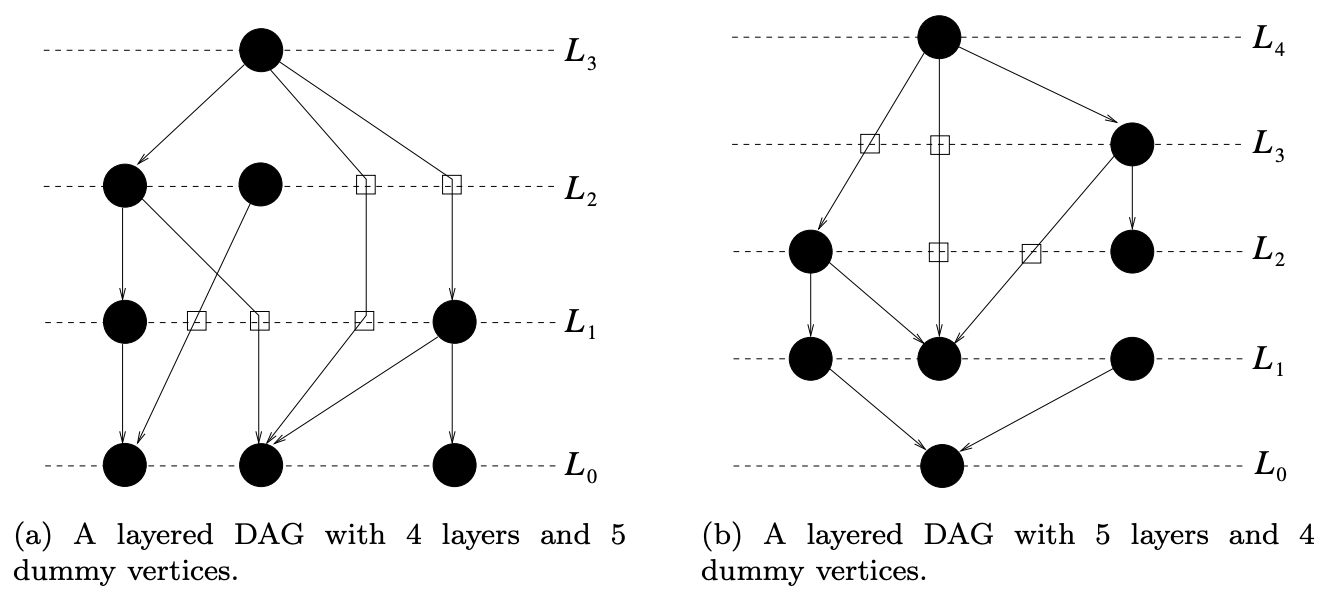
\includegraphics[scale = 0.5]{dummy.png} 
    \end{center}


\end{frame}



% UNCONSTRAINED LAYER ASSIGNMENT
\begin{frame}{Unconstrained Layer Assignment}
    
    \begin{itemize}
        
        \item This is an easy problem with existing solutions.
        \item Depends on modifying classical algorithms used for BFS, DFS and minimum spanning trees.
        \item Algorithms to be studied:

            \begin{itemize}
                
                \item Modified Kahn's algorithm for topological sort
                \item Modified BFS longest path algorithm
                \item Modified DFS
                \item Feasible Spanning Tree/Network Simplex

            \end{itemize}


    \end{itemize}

\end{frame}



% CONSTRAINED LAYER ASSIGNMENT
\begin{frame}{Constrained Layer Assignment}


    \begin{itemize}

        \item In practice, certain constraints are imposed. For example, one such condition is minimising the number of dummy vertices, i.e, $|\mathcal{D}(G, \mathcal{L})|$. In further stages of the Sugiyama framework, too many dummy vertices may produce undesirable criss–crossing of edges.

        \item Algorithms to be studied:

        \begin{itemize}
            
            \item Modified longest path algorithm
            \item Coffman–Graham algorithm
            \item Minimum width layering algorithm
            \item Layering by promotion of vertices
            \item Modified network simplex algorithm
            \item Healy–Nikolov's branch–and–cut algorithm
            \item Layering long edges by edge–splitting

        \end{itemize}

        \item An optional step in the framework to reduce the edge density between adjacent layers, edge crossings and dummy vertices is called \textit{Edge Concentration}.

    \end{itemize}


\end{frame}


% SOURCES AND REFERENCES
\begin{frame}{Sources \& References}
    

    \begin{enumerate}
        
        \item \href{https://graphviz.org/}{AT\&T Graphviz Homepage}
        \item \href{https://gitlab.com/graphviz/graphviz/}{Graphviz Gitlab Repository}
        \item \href{https://cs.brown.edu/people/rtamassi/gdhandbook/}{Handbook of Graph Drawing \& Visualisation – Department of Computer Science, Brown University}
        \item \href{https://www.csd.uoc.gr/~hy583/papers/ch10.pdf}{Layered Drawing of Graphs – Department of Computer Science, University of Crete}
        \item \href{https://www.researchgate.net/publication/220568801_Graph_Layering_by_Promotion_of_Nodes}{Graph Layering by Promotion of Nodes by Nikolov \& Tarassov – Elsevier}

    \end{enumerate}
    

\end{frame}



\end{document}




